\section{Validaci\'on}

El modelo propuesto para recuperar la ecuaci\'on de M\'arkus y H\'azi fue probado mediante la realizaci\'on de una serie de experimentos num\'ericos, destinados a evaluar la capacidad y precisi\'on para simular problemas de flujo multif\'asico con transferencia de calor y cambio de fase. En primer lugar, se obtuvieron soluciones num\'ericas para dos situaciones en las que es posible encontrar una soluci\'on anal\'itica: la estratificaci\'on de un fluido van der Waals en una cavidad con temperatura no uniforme, y la simulaci\'on de un frente de evaporaci\'on. Por otro lado, se simul\'o la generaci\'on de burbujas sobre una placa horizonal calefaccionada, tambi\'en conocido como ebullici\'on heterog\'enea, y se emple\'o este problema para discutir aspectos fundamentales de una simulaci\'on con lattice Boltzmann, como resoluci\'on de grilla y selecci\'on de condiciones de contorno.

\red{condiciones de contorno}
\red{ecuaci\'on de van der Waals}



\subsection{Estratificaci\'on de un fludo van der Waals}
\label{sec:vdWColumnHT}

La \eq{eq:vdw_column_red} permite describir la distribuci\'on unidimensional de densidad en un fluido van der Waals estratificado, de modo que es posible determinar la variaci\'on de densidad en cada fase a partir de una \'unica interfase. Sin embargo, a diferencia de la propuesta de Berberan-Santos \cite{berberan-santos_liquidvapor_2002}, en este caso es admisible que la cavidad presente una distribuci\'onde temperatura no uniforme \cite{fogliatto_simulation_2019}. Esta flexibilidad adicional permite que este mismo problema pueda ser empleado para validar la \lbe{} propuesta. En particular, es sencillo ver que en un caso hidrost\'atico, la \eq{eq:markus_orig} puede expresarse en unidades reducidas como
\begin{equation}
	\dfrac{\partial}{\partial E_r} \left( \lambda \dfrac{\partial T_r}{\partial E_r} \right) = 0.
	\label{eq:markus_1d}
\end{equation}

Por lo tanto, para obtener una soluci\'on compatible con la \lbe{} dada por la \eq{eq:modelo_2d_full}, se completa el algoritmo descripto en la \se{sec:vdw_1d} con la incorporaci\'on de la resoluci\'on de la \eq{eq:markus_1d} usando el esquema de Patankar \cite{patankar_numerical_1980} con condiciones de temperatua fija en los extremos del dominio. De esta manera, actualizando la distribuci\'on de temperatura en el paso 4 y resolviendo de forma iterativa, es posible calcular una distribuci\'on de densidad en un dominio con una distribuci\'on de temperatura que depende del perfil de densidad final. 

Siguiendo el problema detallado en la \se{sec:vdw_1d}, se realizaron simulaciones sobre  una cavidad bidimensional con $H=300$, $L=3$ y condiciones de contorno peri\'odicas en la direcci\'on $x$. En este caso se consider\'o $E_r(H)=10^{-3}$ y una densidad inicial correspondiente al valor cr\'itico ($\rho_r = 1$) con una perturbaci\'on de $\pm 1 \%$.  Para el modelo isot\'ermico se consideraron los mismos factores de relajaci\'on y constates de simulaci\'on, con $M=1$, $G=-1$, $R=1$, $a=0.5$, $b=4$, $\tau_{\rho} = \tau_j=1$, $\tau_{e}^{-1}=\tau_{\zeta}^{-1}=\tau_{q}^{-1}=\tau_{\nu}^{-1}=1.1$, y $\sigma = 0.125$. Por otro lado, para la ecuaci\'on de energ\'ia se emplearon factores de relajaci\'on $q_i = 1$, $c_v = 4$, y par\'ametros libres de la distribuci\'on de equilibrio dados por $\alpha_1 = -1$ y $\alpha_2 = 1$. 

En una primera prueba num\'erica se fij\'o el valor de temperatura de la cara superior en $T_t = 0.99 T_c$, y se realizaron simulaciones para diferentes valores de temperatura en la cara inferior ($T_b$). Las \figs{fig:vdWColumnHT_rhor}{fig:vdWColumnHT_Tr} muestran las distribuciones de densidad y temperatura obtenidas para diferentes valores de $T_b$, donde se observa que, de forma similar a lo que ocurre con el problema isot\'ermico, la fase m\'as densa ocupa la parte inferior del dominio. Sin embargo, en este caso la distribuci\'on de temperatura final no es uniforme o fija, sino que presenta un perfil asociado a una ecuaci\'on de energ\'ia con difusividad t\'ermica constante. Esta restricci\'on determina que el perfil de $T$ presente una variaci\'on significativa en la zona de la fase de vapor, efecto que se acent\'ua con la disminuci\'on de la temperatura de la cara inferior.

La soluci\'n de este problema con lattice Boltzmann reproduce campos macrosc\'opicos con similares caracter\'isticas a los del modelo isot\'ermico, es decir, perfiles de densidad y temperatura similares a la soluci\'on anal\'itica en el seno del fluido, y con una interfase cuyo espesor disminuye con la temperatura. En este caso, la \lbe{} propuesta produce una distribuci\'on de temperatura continua a lo largo de la cavidad, mientras que el espesor no nulo de la interfase no afecta significativamente a la distribuci\'on de $T$ en la zona de la separaci\'on.

\begin{figure}[ht]
	\centering
	\includegraphics[width=0.75\textwidth]{vdWColumnHT_2D/CasoA/rhor_vdWcolumnHT}
	\caption{Distribuci\'on espacial de densidad en una cavidad con diferentes temperaturas en la cara inferior. Las l\'ineas continuas corresponden a simulaciones de lattice Boltzmann.}
	\label{fig:vdWColumnHT_rhor}
\end{figure}

\begin{figure}[ht]
	\centering
	\includegraphics[width=0.75\textwidth]{vdWColumnHT_2D/CasoA/Tr_vdWcolumnHT}
	\caption{Distribuci\'on espacial de temperatura en una cavidad con diferentes temperaturas en la cara inferior. Las l\'ineas continuas corresponden a simulaciones de lattice Boltzmann.}
	\label{fig:vdWColumnHT_Tr}
\end{figure}

El problema de la cavidad constituye un excelente caso para evaluar los efectos de la resoluci\'on espacial en la reproducci\'on de la interfase. En la \fig{fig:vdWColumnHT_rhor_grilla} se muestran los perfiles de densidad reducida simulada con diferentes unidades de grilla en la direcci\'on vertical, usando $T_t = 0.99 \, T_c$ y $T_b = 0.8 \, T_c$. De forma similar a lo que ocurre con la simulaci\'on usando \'unicamente el modelo isot\'ermico, puede confirmarse que si se aplica una adimensionalizaci\'on apropiada (en variables reducidas), la concordancia entre la simulaci\'on y la soluci\'on anal\'itica mejora con el incremento de la resoluci\'on espacial. Es importante destacar que para este caso, el perfil de temperatura presenta un excelente acuerdo con la soluci\'on anal\'itica, como se muestra en la \fig{fig:vdWColumnHT_Tr}, de modo que no se observan cambios apreciables entre las diferentes resoluciones empleadas.

\begin{figure}[ht]
	\centering
	\includegraphics[width=0.75\textwidth]{vdWColumnHT_2D/CasoB/rhor_vdWcolumnHT_grilla}
	\caption{Distribuci\'on espacial de densidad en una cavidad con $T_b = 0.8 \, T_c$, $E_r(H)=10^{-3}$ y diferentes $H$. Las l\'ineas continuas corresponden a simulaciones de lattice Boltzmann.}
	\label{fig:vdWColumnHT_rhor_grilla}
\end{figure}

Como se observ\'o en el cap\'itulo anterior, las constantes de la ecuaci\'on de estado juegan un papel fundamental en la precisi\'on de la simulaci\'on para describir los perfiles de densidad y temperatura a trav\'es de la interfase. Las \figs{fig:vdWColumnHT_rhor_a_eos}{fig:vdWColumnHT_rhor_b_eos} muestran la distribuci\'on de densidad en una cavidad con $T_t = 0.99 \, T_c$ y $T_b = 0.8 \, T_c$, obtenidas con $b=4$ y variando $a$, y con $a=0.5$ pero cambiando $b$. Puede verse que en ambos casos, incrementando $a$ o reduciendo $b$, se reduce el espesor de la interfase en unidades de grilla mientras que se mantienen los perfiles de densidad reducidos en el seno de cada fase. Por otro lado, la disminuci\'on del par\'ametro $b$ aumenta la diferencia entre las densidades de l\'iquido y vapor, mientras que el incremento de $a$ y decremento de $b$ aumenta el gradiente del potencial de interacci\'on. Ambos efectos contribuyen a mejorar la capacidad del modelo \pp{} de reproducir adecuadamente la interfase, lo que induce a las tendencias mostradas en las \figs{fig:vdWColumnHT_rhor_a_eos}{fig:vdWColumnHT_rhor_b_eos}. La consecuencia fundamental radica en que los efectos sobre la soluci\'on adimensional son similares a los observados cuando se incrementa la resoluci\'on de grilla, aunque como ya se mencion\'o previamente, las mejoras de precisi\'on alcanzadas por este camino se encuentran limitadas por restricciones de estabilidad.

\begin{figure}[ht]
	\centering
	\includegraphics[width=0.75\textwidth]{vdWColumnHT_2D/CasoC/rhor_vdWcolumnHT_a_eos}
	\caption{Distribuci\'on espacial de densidad en una cavidad con $T_t = 0.99 \, T_c$ y $T_b = 0.8 \, T_c$. Las l\'ineas continuas corresponden a simulaciones de lattice Boltzmann con $b=4$ y distintos valores de $a$.}
	\label{fig:vdWColumnHT_rhor_a_eos}
\end{figure}

\begin{figure}[ht]
	\centering
	\includegraphics[width=0.75\textwidth]{vdWColumnHT_2D/CasoD/rhor_vdWcolumnHT_b_eos}
	\caption{Distribuci\'on espacial de densidad en una cavidad con $T_t = 0.99 \, T_c$ y $T_b = 0.8 \, T_c$. Las l\'ineas continuas corresponden a simulaciones de lattice Boltzmann con $a=0.5$ y distintos valores de $b$.}
	\label{fig:vdWColumnHT_rhor_b_eos}
\end{figure}
\FloatBarrier



\subsection{Frente de evaporaci\'on}
\label{sec:stefan_d2q9}

Otro caso de estudio relevante para validar modelos de lattice Boltzmann con cambio de fase consiste en la simulaci\'on de un frente de evaporaci\'on, tambi\'en conocido como flujo de Stefan unidimensional \cite{alexiades_mathematical_1993}. Como se muestra en la \fig{fig:Stefan_cavity}, el problema puede describirse como una cavidad unidimensional, con un extremo abierto, e inicialmente llena de l\'iquido a temperatura de saturaci\'on $T_s$. Si la temperatura del extremo cerrado ($T_w$) supera el valor de saturaci\'on, es decir $T_w > T_s$, comienza a producirse un cambio de fase en esta zona, y la evoluci\'on de la posici\'on de la interfase puede aproximarse anal\'iticamente. 

\begin{figure}[ht]
	\centering
	\includegraphics[width=0.75\textwidth]{Stefan/Stefan}
	\caption{Definici\'on del problema de flujo de Stefan}
	\label{fig:Stefan_cavity}
\end{figure}

El libro de Alex\'iades y Solomon \cite{alexiades_mathematical_1993} contiene una descripci\'on detallada sobre la obtenci\'on de soluciones anal\'iticas para diferentes problemas de cambio de fase, de modo que aqu\'i s\'olo se muestra un breve resumen del problema a evaluar. En el caso de inter\'es, la fase de vapor puede considerarse en reposo, de modo que la ecuaci\'on de energ\'ia en esta regi\'on se reduce a 
\begin{equation}
	\dfrac{\partial T}{\partial t} = \chi \dfrac{\partial^2 T}{\partial x^2}, \qquad 0 < x < x_i(t),
\end{equation}
donde $x_i(t)$ corresponde a la posici\'on de la interfase que cambia en el tiempo. Si se imponen condiciones de contorno de Dirichlet para la regi\'on de vapor, es decir
\begin{subequations}
	\begin{equation}
		T(x=0,t) = T_w
	\end{equation}
	\begin{equation}
		T(x=x_i(t),t) = T_s,
	\end{equation}	
\end{subequations}
entonces el problema es resoluble si se considera una condici\'on de salto de energ\'ia sobre la interfase:
\begin{equation}
	\rho_g u_i h_{fg} = -\lambda_g \left.\dfrac{\partial T}{\partial x} \right|_{x=x_i(t)},
\end{equation}
donde $u_i=dx_i/dt$, $h_{fg}$ es el calor latente y $\lambda_g$ la conductividad t\'ermica de la fase de vapor. Con estas aproximaciones, la posici\'on de la interfase en funci\'on del tiempo puede estimarse como:
\begin{equation}
	x_i(t)=2\beta \sqrt{\chi_lt},
	\label{eq:stefan_int}
\end{equation},
donde $\chi_l$ corresponde a la difusividad t\'ermica de la fase l\'iquida y $\beta$ satisface la siguiente ecuaci\'on trascendental:
\begin{equation}
	\beta \mbox{e}^{\beta^2}\mbox{erf}(\beta)=\dfrac{c_{pg}(T_w-T_s)}{h_{fg}\sqrt{\pi}} = \dfrac{St}{\sqrt{\pi}}.
	\label{eq:stefan_beta}
\end{equation}

En la \eq{eq:stefan_beta} $c_{pg}$ es el calor espec\'ifico a presi\'on constante de la fase de vapor y $St$ se conoce como el n\'umero de Stefan. 

La descripci\'on de la din\'amica del frente de vapor asume que la temperatura de la interfase y de toda la regi\'on de fluido es igual a $T_s$. Por otro lado, la fase de vapor se encuentra en reposo, y el movimiento de la interfase desplaza la columna de l\'quido con velocidad uniforme (pero no constante en el tiempo) hacia el extremo abierto del dominio. Estas hip\'otesis sobre la soluci\'on anal\'itica imponen restricciones al momento de emplear este problema como caso de prueba de un modelo de lattice Boltzmann, aunque ya ha sido utilizado satisfactoriamente por Safari y colaboradores \cite{safari_consistent_2014} para validar un modelo t\'ermico de la familia phase-field. Sin embargo, a diferencia de un modelo phase-field, en un modelo \pp{} no es posible fijar la temperatura de la interfase, por lo que es necesario recurrir a una condici\'on de simulaci\'on que permita sobreponer parcialmente esta restricci\'on. En particular, si se recupera una ecuaci\'on de energ\'ia con $\chi$ constante en cada fase, entonces la construcci\'on de un caso computacional donde $\rho_l \gg \rho_g$ produce $\lambda_l \gg \lambda_g$, y por lo tanto la temperatura sobre la interfase se asemeja a la del extremo del dominio computacional $T_s$.

La evoluci\'on de un frente de evaporaci\'on se simul\'o con lattice Boltzmann usando un dominio de $L=600$ unidades de grilla en la direcci\'on $x$ y s\'olo $H=3$ en la direcci\'on $y$, ya que no se observaron diferencias significativas en simulaciones realizadas sobre grillas con m\'as elementos en la direcci\'on peri\'odica. La cantidad elegida de nodos en la direcci\'on principal reduce efectos de la condici\'on de contorno en el extremo abierto sobre el interior del dominio. En todos los casos se impusieron condiciones de temperatura fija en los extremos del dominio con $T(L) = 0.8 \, T_c$, de no deslizamiento en $x=0$, y de flujo saliente (\emph{outflow}) para densidad y velocidad en $x=L$ \cite{lou_evaluation_2013}. En esta \'ultima condici\'on, los valores de $\rho$ y $\bm{u}$ sobre los nodos de la frontera se obtienen a partir de una interpolaci\'on considerando nodos del interior y una velocidad de advecci\'on. De esta forma, las componentes de $\bm{f}$ son actualizadas despu\'es del paso de \emph{streaming} para satisfacer los momentos macrosc\'opicos extrapolados.

Las constantes de simulaci\'on empleadas en las \lbe{} hidrodin\'amica y de energ\'ia se encuentran en las \tabs{}{} respectivamente \red{poner tablas}. Inicialmente, el dominio se encuentra a temperatura uniforme $T_r = 0.8$, y la distribuci\'on de densidad es uniforme e igual a la de coexistencia de la fase l\'iquida a $T_r = 0.8$. Si se deja evolucionar un sistema con esta configuraci\'on, inicialmente se produce una zona de vapor en $x=0$ sin necesidad de incluir un disparador adicional, como puede ser una peque\~na regi\'on de vapor, y la posici\'on de la interfase de desplaza hasta alcanzar $x=L$. La \fig{fig:Stefan_m1_1} muestra la posici\'on de la interfase calculada usando diferentes valores de $T_w$, lo cual se refleja en distintos n\'umeros de Stefan. 

\begin{figure}[ht]
	\centering
	\includegraphics[width=0.75\textwidth]{Stefan/2D/CasoA/Stefan_m1_1}
	\caption{Posici\'on del frente de evaporaci\'on para diferentes n\'umeros de Stefan, con $\alpha_1 = -1$, $\alpha_2=1$ y $q_{\chi} = 1.8$. Las l\'ineas s\'olidas corresponden a las simulaciones con lattice Boltzmann}
	\label{fig:Stefan_m1_1}
\end{figure}

Las soluciones anal\'iticas fueron estimadas usando $h_{fg}=h_g-h_l$, donde la entalp\'ia de cada fase puede determinarse anal\'iticamente a partir de la ecuaci\'on de estado de van der Waals \cite{markus_simulation_2011}:
\begin{equation}
	h = \left( \dfrac{3}{2} \dfrac{1}{1-b\rho} \right)RT - 2b\rho.
	\label{eq:hfg_vdw}
\end{equation}

La evoluci\'on de la interfase mostrada en la \fig{Stefan_m1_1} indica que el modelo propuesto puede reproducir satisfactoriamente la estimaci\'on dada por las \eqs{eq:stefan_int}{eq:stefan_beta}, lo que implica que la transferencia de masa a trav\'es de las interfase puede ser recuperada correctamente cuando el cambio de fase est\'a governado por una ecuaci\'on de estado, sin necesidad de reconstruir la interfase o de efectuar aproximaciones adicionales.

En este punto, y tomando como base los resultados del frente de evaporaci\'on, es posible mostrar que la \lbe{} propuesta para recuperar la ecuaci\'on de energ\'ia tiene la capacidad de reducir posibles restricciones de estabilidad asociadas al uso de valores grandes de $q_{\chi}$, ya que como se aprecia en la \eq{eq:modelo_2d_chi}, la difusividad t\'ermica tambi\'en puede ser ajustada mediante $\alpha_1$ y $\alpha_2$. Para ilustrar esta caracter\'istica, se realizaron simulaciones del frente de evaporaci\'on usando $\alpha_1=-2$, $\alpha_2=2$ y $q_{\chi}=1.7143$, lo que formalmente reproduce la misma difusividad t\'ermica que $\alpha_1=-1$, $\alpha_2=1$ y $q_{\chi}=1.8$, y por lo tanto, el mismo resultado f\'isico. Como se aprecia en la \fig{fig:Stefan_m2_2}, la evoluci\'on del frente de evaporaci\'on no se distingue de aquella obtenida mediante otro conjunto de par\'ametros (\fig{fig:Stefan_m1_1}), lo que indica que la difusividad t\'ermica recuperada es la misma en ambos casos. Esta capacidad de usar diferentes factores de relajaci\'on para lograr un mismo valor de $\chi$ puede ser utilizada para compensar simulaciones num\'ericamente inestables.

\begin{figure}[ht]
	\centering
	\includegraphics[width=0.75\textwidth]{Stefan/2D/CasoB/Stefan_m2_2}
	\caption{Posici\'on del frente de evaporaci\'on para diferentes n\'umeros de Stefan, con $\alpha_1 = -2$, $\alpha_2=2$ y $q_{\chi} = 1.7143$. Las l\'ineas s\'olidas corresponden a las simulaciones con lattice Boltzmann}
	\label{fig:Stefan_m2_2}
\end{figure}










\subsection{Ebullici\'on heterog\'enea}

El modelo propuesto es capaz de reproducir con precisi\'on la estratificaci\'on de un fluido van der Waals con transferencia de calor y la evoluci\'on de un frente de evaporaci\'on. Por otro lado, la generaci\'on, crecimiento y partida de una burbuja sobre  una superficie calefaccionada constituye un excelente caso de prueba para completar la validaci\'on de un modelo de lattice Boltzmann t\'ermico. En este problema no s\'olo es posible agrupar toda la fenomenolog\'ia analizada previamente en un \'unico caso de estudio, sino que tambi\'en es posible emplear expresiones anal\'iticas para estimar par\'ametros globales como di\'ametro de partida. Por lo tanto, la simulaci\'on de ebullici\'on heterog\'enea provee un mecanismo adicional para evaluar la precisi\'on del modelo, mientras que puede ser usada para clarificar aspectos que no suelen encontrarse en la literatura espec\'ifica, como resoluci\'on de grilla y consistencia de lattice Boltzmann (como m\'etodo num\'erico) en un problema f\'isicamente complejo.

Siguiendo el objetivo de reproducir la fenomenolog\'ia b\'asica de ebullici\'on heterog\'enea, se realizaron simulaciones en una grilla bidimensional similar a la utilizada en la \se{sec:vdWColumnHT}, pero con temperaturas de pared iguales al valor de saturaci\'on, es decir $T_t = T_b = T_s = 0.8 \, T_c$.  Por otro lado, en el centro de la cara inferior se incorpor\'o una peque\~na secci\'on de longitud $L_h$ con temperatura $T_w > T_s$, como se muestra esquem\'aticamente en la \fig{fig:hetb_esquema}. 

\begin{figure}[ht]
	\centering
	\includegraphics[width=0.5\textwidth]{HetBoiling/Heater}
	\caption{Esquema del dominio usado para simular el problema de ebullici\'on heterog\'enea.}
	\label{fig:hetb_esquema}
\end{figure}

Las simulaciones fueron inicializadas con temperatura uniforme $T_s$, $\rho = \rho_l$ para $y\leq H$ y $\rho = \rho_g$ para $y > H$, donde $\rho_l$ y $\rho_g$ son las densidades de equilibrio de las fases l\'iquida y gaseosa a $T_s$ respectivamente. Salvo que se mencione expl\'icitamente lo contrario, se utilizaron las constantes de simulaci\'on detalladas en la \tb{tab:hetb_prop}.

\begin{table}[ht]
	\centering
    \begin{tabular}{c c}
	    \toprule
        \bf Propiedad & \bf Valor \\
        \midrule
        $\tau_{\rho}^{-1}$, $\tau_{j}^{-1}$ & 1.0\\
        $\tau_{e}^{-1}$, $\tau_{\zeta}^{-1}$, $\tau_{q}^{-1}$ & 1.1 \\
        $\tau_{\nu}^{-1}$ & 1.1 \\
		a & 1 \\
		b & 4 \\
		$q_{0-2}$, $q_4$, $q_{6-8}$ & 1.0 \\
		$q_{\chi}$ & 1.5 \\
		$\alpha_1$ & -1 \\
		$\alpha_2$ & 1 \\
		$c_v$ & 4 \\
        \bottomrule
	\end{tabular}
	\caption{Constantes de simulaci\'on para el problema de ebulluci\'on heterog\'enea.}
	\label{tab:hetb_prop}
\end{table}  
\FloatBarrier


\subsubsection{Independencia de grilla}

Las discretizaciones espacial y temporal tiene un rol fundamental en la estabilidad y precisi\'on de las simulaciones. Aunque el concepto de refinamiento de malla parece natural (en muchos casos) dentro de las t\'ecnicas num\'ericas tradicionales, en lattice Boltzmann es necesario prestar especial atenci\'on para poder describir adecuadamente el problema deseado, ya que como se mencion\'o en el \chap{chap:fundamentos}, las propiedades del fluido dependen del tama\~no de la unidad de grilla. Debido a esta propiedad peculiar, existen dos metodolog\'ias ampliamente aceptadas para evaluar los resultados de una simulaci\'on \cite{kruger_lattice_2017}: calcular la correspondencia entre unidades de grilla y unidades f\'isicas, o bien preservar n\'umeros adimensionales relevantes. En el caso de flujos multif\'asicos la primera alternativa suele ser complicada, de modo que, aprovechando las ventajas de la adimensionalizaci\'on usada en los ejemplos de validaci\'on anteriores (es decir, en unidades reducidas), es preferible optar por el segundo camino.

El an\'alisis adimensional de las ecuaciones macrosc\'opicas para flujo multif\'asico con transferencia de calor muestra que es posible construir un grupo de par\'ametros adimensionales \'utiles para problemas t\'ipicos de ebullici\'on \cite{ajaev_modeling_2006, hua_numerical_2007}:
\begin{equation}
	Re = \dfrac{\rho_l g^{1/2} D^{3/2}}{\mu_l}, \qquad
	Bo = \dfrac{\rho_l g D^2}{\kappa}, \qquad
	Pr = \dfrac{\nu}{\alpha}, \qquad
	Ja = \dfrac{c_v}{h_{fg}}(T_w-T_s),
	\label{eq:num_adim_hetb}
\end{equation}
donde $Re$, $Bo$, $Ja$ y $Pr$ son los n\'umeros de Reynolds, Bond, Jacob y Prandtl respectivamente. En la \eq{eq:num_adim_hetb} $D$ corresponde a una dimension caracter\'istica, $\mu_l$ a la viscosidad din\'amica de la fase l\'iquida, $\kappa$ a la tensi\'on superficial, y $T_w$ y $T_s$ corresponden a la temperatura sobre la pared y en el seno del fluido, respectivamente. 

En las simulaciones de lattice Bolzmann con modelos \pp{} ciertas propiedades macrosc\'opicas como tensi\'on superficial y calor latente no pueden imponerse expl\'icitamente, sino que se obtienen como un resultado directo de la simulaci\'on. Por lo tanto, la comparaci\'on entre simulaciones realizadas sobre diferentes mallas que comparten los mismos n\'umeros adimensionales contribuye significativamente a determinar el rango de validez de los modelos empleados. Adem\'as, como las ecuaciones macrosc\'opicas objetivo se recuperan s\'olo hasta un cierto orden de aproximaci\'on, este tipo de an\'alisis constituye una manera adicional de verificar si los t\'erminos de alto orden de la expansi\'on de Chapman-Enskog pueden ser efectivamente despreciados.

Por otro lado, de manera similar a lo que ocurre con otros modelos de interfase difusa, el espesor de la misma ($d_i$) influye significativamente en el resultado final de la simulaci\'on \cite{ding_diffuse_2007}, de modo que debe ser suficientemente peque\~no comparado con las dimendiones principales del fen\'omeno simulado. En el presente caso, los resultados num\'ericos de las Secciones~\ref{sec:vdw_1d} y \ref{sec:vdWColumnHT} muestran que el espesor de la interfase, en unidades de grilla, puede ser controlado mediante las constantes de la ecuaci\'on de estado. 

Estos criterios de an\'alisis pueden cumplirse si se aplica un estudio de independencia de grilla de dos pasos. En primer lugar, es necesario realizar un conjunto de simulaciones de un mismo problema sobre diferentes grillas, pero que compartan los n\'umeros adimensionales dados por la \eq{eq:num_adim_hetb} y preserven el espesor de interfase reducido (es decir, $d_i/D$) a trav\'es de una selecci\'on adecuada de las constantes de la ecuaci\'on de estado. Como se mencion\'o previamente, las ecuaciones macrosc\'opicas se recuperan adecuadamente si se obtienen resultados similares con diferentes grillas. Por otro lado, el segundo paso consiste en realizar simulaciones sobre diferentes grillas con los mismos par\'ametros adimensionales, pero esta vez fijando el espesor de la interfase en unidades de grilla (p\'arametros la ecuaci\'on de estado iguales en cada simulaci\'on). \newline

Para llevar a cabo el primer paso de la prueba de independencia de grilla se seleccionaron un conjunto de constantes de van der Waals que conducen a un perfil de densidad reducida, y por lo tanto adimensional, que permanece invariante a la cantidad de unidades de grilla. Esta selecci\'on se llev\'o a cabo tomando como base el problema de estratificaci\'on utilizado en la \se{sec:vdw_1d}: una vez calculado el perfil adimensional sobre coordenadas normalizadas en un primer caso de referencia, se selecciona la altura $H$ para el siguiente y, conservando $E_r(H)$, se realizan simulaciones para distintos valores de $a$ y $b$ hasta lograr la mejor aproximaci\'on en media cuadr\'atica de los perfiles reducidos en la zona de la interfase. Esta metodolog\'ia  de c\'alculo y comparaci\'on se implement\'o en Python, haciendo uso del m\'odulo scipy.optimize y del m\'edodo de Nelder-Mead para acelerar la b\'usqueda de las constantes.

Una vez seleccionado el conjunto de constantes $\{(a,b)\}$, se obtuvieron para cada caso los valores de tensi\'on superficial y calor latente mediante experimentos de ley de Laplace (\red{ver Ap\'endice}) y con la \eq{eq:hfg_vdw} respectivamente. De esta manera, fue posible construir los casos detallados en la \tb{tab:gridindep_step1}.
\begin{table}[ht]
	\centering
    \begin{tabular}{c c c c c c c}
	    \toprule
        \bf Grilla ($L\times H$) & $\bm{a}$ & $\bm{b}$ & $\bm{L_h}$ & $\bm{g}$ & $\bm{\tau_{\nu}^{-1}}$ & $\bm{q_{\chi}}$ \\
        \midrule
		300 $\times$ 500   & 1 & 4 & 6 & $8\cdot 10^{-6}$ & 1.30 & 1.55 \\
		600 $\times$ 1000  & 0.49 & 8.2 & 12 & $9.54\cdot 10^{-7}$ & 1.31 & 1.56 \\		
        \bottomrule
	\end{tabular}
	\caption{Par\'ametros de simulaci\'on para el primer paso de prueba de independencia de grilla.}
	\label{tab:gridindep_step1}
\end{table}  

En la \fig{fig:bubble2D_step1} se muestran capturas de la interfase durante el proceso de formaci\'on y desprendimiento de una burbuja, obtenidas para diferentes grillas a tiempos adimensionales definidos como $t^* = t \sqrt{g/D}$. Puede verse que si los par\'ametros de simulaci\'on son seleccionados adecuadamente, conservando los n\'umeros adimensionales de la \eq{eq:num_adim_hetb} y el espesor adimensional de la interfase, los resultados num\'ericos son pr\'acticamente independientes de la resoluci\'on de grilla. Este resultado verifica que las ecuaciones macrosc\'opicas se recuperan de acuerdo a lo esperado, al menos para las condiciones de simulaci\'on utilizadas.

\begin{figure}[htb]
    \centering
    \begin{subfigure}[t]{0.45\textwidth}
        \centering
        \includegraphics[width=0.95\textwidth]{Imagenes/HetBoiling/GridIndep_1/20}
        \caption{$t^*=0.65$}
    \end{subfigure}
    \begin{subfigure}[t]{0.45\textwidth}
        \centering
        \includegraphics[width=0.95\textwidth]{Imagenes/HetBoiling/GridIndep_1/60}
        \caption{$t^* = 1.96$}
    \end{subfigure}
    \begin{subfigure}[t]{0.45\textwidth}
        \centering
        \includegraphics[width=0.95\textwidth]{Imagenes/HetBoiling/GridIndep_1/90}
        \caption{$t^* = 2.94$}
    \end{subfigure}    
    \begin{subfigure}[t]{0.45\textwidth}
        \centering
        \includegraphics[width=0.95\textwidth]{Imagenes/HetBoiling/GridIndep_1/130}
        \caption{$t^* = 4.25$}
    \end{subfigure}    
    \caption{Formaci\'on y desprendimiento de una burbuja para diferentes grillas y constantes de van der Waals: ($300 \times 500$, $a=1$, $b=4$) en l\'inea negra, y ($600 \times 1000$, $a=0.49$, $b=8.2$) en l\'inea roja.}
    \label{fig:bubble2D_step1}
\end{figure}

En el segundo paso del an\'alisis de independencia de grilla se busc\'o evaluar el comportamiento de una figura de m\'erito global de la simulaci\'on, como el di\'ametro de partida. Para ello se comenz\'o el proceso con un caso base (A) y se construyeron los restantes manteniendo los n\'umeros adimensionales principales usando $a=1$ y $b=4$, es decir, fijando el espesor de la interfase en unidades de grilla. Los resultados obtenidos para este paso se encuentran resumidos en la \tb{tab:gridindep_step2}, donde adem\'as puede verse que el di\'ametro de partida converge con orden 2.8 usando el criterio de convergencia de ASME \cite{freitas_asmes_2003}. Adem\'as, la grilla empleada en el Caso B provee una buena aproximaci\'on del resultado extrapolado, por lo que ser\'a utilizada en simulaciones posteriores.

\begin{table}[ht]
	\centering
    \begin{tabular}{c c c}
	    \toprule
        \bf Caso & \bf Grilla ($L\times H$) & $\bm{D_{eq}/L}$  \\
        \midrule
		A & 300  $\times$ 500  &  0.2209 \\
		B & 600  $\times$ 1000 &  0.2091 \\		
		C & 1200 $\times$ 2000 &  0.2064 \\		
		Extrapolado &          &  0.2039 \\		
        \bottomrule
	\end{tabular}
	\caption{An\'alisis de independencia de grilla para el di\'ametro de partida equivalente.}
	\label{tab:gridindep_step2}
\end{table} 


\subsubsection{Condici\'on de borde para $T$}

La elecci\'on de condiciones de contorno para esquemas de lattice Boltzmann constituye un aspecto fundamental de la simulaci\'on, ya que el tratamiento de las fronteras t\'ermicas influye significativamente en los procesos de formaci\'on, crecimiento y desprendimiento de burbujas. En este aspecto, suele ocurrir que modelos t\'ermicos v\'alidos sean descartados simplemente por una elecci\'on incorrecta de las condiciones de contorno. En general este aspecto no se encuentra documentado con claridad en la literatura asociada a modelos t\'ermicos, por lo que se mostrar\'a una breve descripci\'on.

Algunas de las alternativas propuestas para recuperar las componentes desconocidas de la funci\'on de distribuci\'on $g$ despu\'es del paso de \emph{streaming} se conocen como m\'etodo de equilibrio \cite{kruger_lattice_2017}, m\'etodo de extrapolaci\'on \cite{guo_extrapolation_2002} y m\'etodo de Inamuro \cite{inamuro_lattice_2002}. En el m\'etodo de equilibrio, todas las componentes de la funci\'on de distribuci\'on sobre nodos de la frontera son reemplazadas por su valor de equilibrio a la temperatura deseada, es decir, $\feq{g} = \bm{M}^{-1}\feq{n}(T_w)$.  Por otro lado, en el m\'etodo de extrapolaci\'on se incorporan las componentes de no equilibrio a trav\'es de la extrapolaci\'on desde nodos interiores:
\begin{equation}
	g_{\alpha}(\bm{x}_b,t) = g_{\alpha}^{eq}(T_b, \bm{u}_b) + \left[ g_{\alpha}(\bm{x}_f,t) - g_{\alpha}^{eq}(T_f, \bm{u}_f)\right],
\end{equation}
donde la contribuci\'on de no equilibrio sobre el nodo de frontera en $\bm{x}_b$ est\'a determinada por las del nodo de fluido m\'as cercano, $\bm{x}_f$, ubicado sobre la normal a la frontera. Finalmente, el m\'etodo de Inamuro propone reemplazar s\'olo las componentes desconocidas por su valor de equilibrio correspondiente, y posteriormente escalearlas con el mismo factor para preservar el valor de temperatura deseado sobre la pared.

La \fig{fig:bubble2D_bnd} muestra contornos de densidad obtenidos de simulaciones con diferentes condiciones de contorno par $T$. Los gr\'aficos fueron obtenidos a $t=15000\,\delta_t$ en una grilla de $600\times 1000$ nodos. 

\begin{figure}[htb]
    \centering
    \begin{subfigure}[t]{0.45\textwidth}
        \centering
        \includegraphics[width=0.95\textwidth]{Imagenes/HetBoiling/Borde/density_inamuro_fd}        
        \caption{Inamuro}
	    \label{fig:bubble2d_inamuro}        
    \end{subfigure}
    \begin{subfigure}[t]{0.45\textwidth}
        \centering
        \includegraphics[width=0.95\textwidth]{Imagenes/HetBoiling/Borde/density_extrapolation_fd}
        \caption{Extrapolaci\'on}
    \end{subfigure}
    \begin{subfigure}[t]{0.45\textwidth}
        \centering
        \includegraphics[width=0.95\textwidth]{Imagenes/HetBoiling/Borde/density_equilibrium_fd}
        \caption{Equilibrio}
    \end{subfigure}    
    \caption{Desprendimiento de una burbuja para diferentes condiciones de contorno para la temperatura. La l\'inea roja indica la posici\'on de la frontera obtenida usando un esquema de diferencias finitas para la ecuaci\'on de energ\'ia.}
    \label{fig:bubble2D_bnd}
\end{figure}

Como puede observarse en la \fig{fig:bubble2d_inamuro}, la condici\'on de Inamuro lleva a la formaci\'on de una burbuja y posterior rompimiento del cuello, lo cual es consistente con simulaciones realizadas usando un esquema de diferencias finitas para la temperatura, como el descripto en \cite{li_lattice_2015}. Sin embargo, esta tendencia no se observa para las condiciones de equilibrio o extrapolaci\'on. El origen de este problema se evidencia en la \fig{fig:hetb_T_cdb}, donde se muestran los perfiles de temperatura desde el centro de la regi\'on calefaccionada , sobre la coordenada vertical, para $t=400\,\delta_t$. Si bien todas las condiciones de contorno recuperan adecuadamente el valor de temperatura deseado sobre la pared, las componentes de la funci\'on de distribuci\'on $\bm{g}$ son distintos en cada caso. Esta diferencia se propaga hacia el seno del fluido durante el paso de \emph{streaming}, y conduce a una sobreestimaci\'on de la temperatura cerca de la pared para los m\'etodos de equilibrio y extrapolaci\'on. De esta forma, este incremento artificial de $T$ evita el rompimiento del cuello, y por lo tanto no se produce el desprendimiento de la burbuja.
\begin{figure}[ht]
	\centering
	\includegraphics[width=0.75\textwidth]{HetBoiling/Borde/T_cdb_color}
	\caption{Perfiles de temperatura en $x=300$ y $t=400\,\delta_t$, correspondientes a distintas condiciones de contorno para $T$.}
	\label{fig:hetb_T_cdb}
\end{figure}


\subsubsection{Representaci\'on de $\nabla T$}

El t\'ermino de fuente dado por la \eq{eq:model2D_hs} requiere del c\'omputo adicional del gradiente de temperatura, de modo que un primer m\'etodo consiste en implementar este c\'alculo mediante un esquema de diferencias finitas. Sin embargo, es posible estimar $\nabla T$ mediante la \eq{eq:gradT_2d}, incorporando s\'olo la definici\'on local de la funci\'on de distribuci\'on y su valor de equilibrio, lo cual se convierte en una ventaja significativa en procesamiento distribuido. De esta manera, con el objetivo de verificar esta propuesta, se simul\'o la formaci\'on de una burbuja sobre una grilla de $600\times 1000$ nodos (Caso B de la \tb{tab:gridindep_step2}) usando ambos esquemas para calcular $\nabla T$. Como se observa en la \fig{fig:bubble2D_gradT}, no se observan diferencias significativas en la forma de la interfase para diferentes instantes de tiempo. Por lo tanto, la aproximaci\'on a primer orden de $\varepsilon$ dada por la \eq{eq:gradT_2d} constituye una excelente alternativa, sobre todo para aquellos casos en los que los recursos computacionales son limitados.

\begin{figure}[htb]
    \centering
    \begin{subfigure}[t]{0.45\textwidth}
        \centering
        \includegraphics[width=0.95\textwidth]{Imagenes/HetBoiling/gradT/20}   
        \caption{$t^*=0.58$}     
    \end{subfigure}
    \begin{subfigure}[t]{0.45\textwidth}
        \centering
        \includegraphics[width=0.95\textwidth]{Imagenes/HetBoiling/gradT/30}
        \caption{$t^*=0.87$}
    \end{subfigure}
    \begin{subfigure}[t]{0.45\textwidth}
        \centering
        \includegraphics[width=0.95\textwidth]{Imagenes/HetBoiling/gradT/45}
        \caption{$t^*=1.3$}
    \end{subfigure}    
    \begin{subfigure}[t]{0.45\textwidth}
        \centering
        \includegraphics[width=0.95\textwidth]{Imagenes/HetBoiling/gradT/60}
        \caption{$t^*=1.73$}
    \end{subfigure}        
    \caption{Formaci\'on y desprendimiento de una burbuja para diferentes aproximaciones de $\nabla T$. En l\'inea roja se muestra la interfase calculada con diferencias finitas, y en l\'inea negra usando la \eq{eq:gradT_2d}.}
    \label{fig:bubble2D_gradT}
\end{figure}



\subsubsection{Di\'ametro de partida equivalente}

En las \'ultimas d\'ecadas, se han desarrollado diferentes correlaciones capaces de estimar caracter\'sticas macrosc\'opicas del fen\'omeno de ebullici\'on heterog\'enea, como di\'ametro de partida de las burbujas. Una correlaci\'on popular para estimar el di\'ametro de partida desde una superficie horizontal calefaccionada fue propuesta por Fritz \cite{fritz_berechnung_1935}:
\begin{equation}
	D_p = 0.0208 \theta_c \left[ \dfrac{\kappa}{g(\rho_l-\rho_g)} \right]^{0.5},
	\label{eq:g_fritz}
\end{equation}
donde $D_p$ es el di\'ametro de partida y $\theta_c$ el \'angulo de contacto. Recientemente, Phan y colaboradores propusieron otra expresi\'on dada por:
\begin{equation}
	D_p = 1.94 \left[ \dfrac{\kappa}{g(\rho_l-\rho_g)} \right]^{0.5} \left( \dfrac{\rho_l}{\rho_g} \right)^{-0.5} \left( \dfrac{\rho_l}{\rho_g} -1\right)^{1/3} \tan\theta_c^{1/6}.
	\label{eq:g_phan}
\end{equation}

Estas correlaciones sirven como ejemplo para destacar que, independientemente de los factores que dependen de la densidad de cada fase, \'angulo de contacto o tensi\'on superficial, la mayor\'ia de las correlaciones tienen en com\'un que el di\'ametro de partida cambia proporcionalmente con $g^{-0.5}$. Por lo tanto, como los modelos analizados hasta este punto corresponden a 2 dimensiones, y por ende no es posible realizar una comparaci\'on directa con las \eqs{eq:g_fritz}{eq:g_phan}, s\'i es factible usar esta dependencia con $g$ como paso adicional para verificar el comportamiento de la \lbe{} propuesta.

En la \fig{fig:dvsg_2d} el di\'ametro equivalente de partida para una grilla de $600\times 1000$ nodos en funci\'on de $g$. Puede verse que los resultados num\'ericos obtenidos con el modelo t\'ermico propuesto presentan un excelente acuerdo con las caracter\'isticas comunes de las correlaciones.

\begin{figure}[ht]
	\centering
	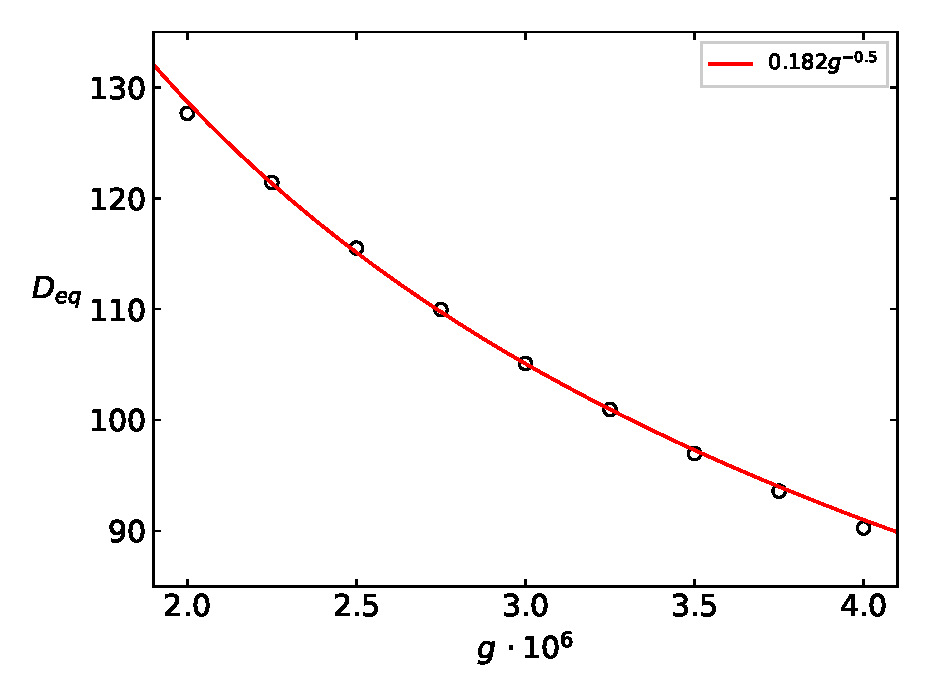
\includegraphics[width=0.75\textwidth]{HetBoiling/Diametro/d_vs_g}
	\caption{Di\'ametro de partida equivalente en funci\'on de $g$.}
	\label{fig:dvsg_2d}
\end{figure}

\red{rehacer esta figura}







\section{Conclusiones}

En este cap\'itulo se introdujo un nuevo esquema de lattice Boltzmann en dos dimensiones, con dos funciones de distribuci\'on y operador de colisi\'on MRT, destinado a la resoluci\'on de flujos multif\'asicos con transferencia de calor. Este modelo acopla una \lbe{} de la familia \pp{} para resolver las ecuaciones hidrodin\'amicas, junto con una ecuaci\'on modificada para el transporte de energ\'ia.

A diferencia de los esquemas de lattice Boltzmann tradicionales, la estrategia propuesta introduce una adecuada definici\'on de la distribuci\'on de equilibrio directamente en el espacio de momentos, con par\'ametros libres que pueden usarse para ajustar la difusividad t\'ermica recuperada. Adem\'as, el an\'alisis de Chapman-Enskog muestra que cuando esta distribuci\'on de equilibrio se emplea junto con una matriz de relajaci\'on con coeficientes extra diagonales no nulos, adecuadamente definidos, la ecuaci\'on de energ\'ia macrosc\'opica se recupera sin t\'erminos adicionales hasta la escala de expansi\'on analizada. De esta forma, no es necesario aplicar correcciones expl\'icitas a los t\'erminos de fuente o a la distribuci\'on post-colisi\'on, usualmente usadas para eliminar los efectos relacionados con la simulaci\'on de ecuaciones escalares de advecci\'on-difusi\'on usando esquemas lattice Boltzmann cl\'asicos.

El modelo propuesto es capaz de reproducir problemas num\'ericos con soluciones anal\'iticas, como distribuci\'on de temperatura y densidad en un fluido van der Waals estratificado, as\'i como la evoluci\'on de la interfase en un problema de Stefan unidimensional. En el primer caso, el modelo es capaz de calcular adecuadamente las distribuciones en el centro del fluido y la posici\'on de la interfase para diferentes condiciones de contorno. De forma similar a lo observado en el caso isot\'ermico, se observa consistencia del m\'etodo en unidades reducidas. En la segunda prueba, la evoluci\'on de la posici\'on de la interfase pudo ser reproducida satisfactoriamente usando diferentes combinaciones de constantes de equilibrio y par\'ametros de relajaci\'on que conducen a una misma difusividad t\'ermica, lo que evidencia el cumplimiento del comportamiento previsto por la expansi\'on de Chapman-Enskog.

Por otro lado, se analiz\'o la consistencia y orden de convergencia del modelo propuesto mediante la simulaci\'on de generaci\'on de burbujas sobre una superficie horizontal calefaccionada. Para ello, se aplic\'o una evaluaci\'on de independencia de grilla de dos pasos, tomando como base la reproducci\'on de n\'umeros adimensionales caracter\'isticos. En primer lugar, se realizaron simulaciones sobre diferentes grillas, conservando estos par\'ametros junto con el espesor de interfase adimensional. En este caso, no se observaron diferencias significativas en la evoluci\'on de la interfase entre las distintas simulaciones, lo que constituye un claro indicio de que las ecuaciones macrosc\'opicas se recuperan seg\'un lo esperado. Por otro lado, se realiz\'o un segundo conjunto de simulaciones sobre diferentes grillas, conservando los mismos n\'umeros adimensionales relevantes pero conservando el espesor de interfase en unidades de grilla. En este caso, el di\'ametro de partida adimensional converge con orden 2.18.

El problema de ebullici\'on heterog\'enea sirvi\'o adem\'as que la elecci\'on del m\'etodo usado para aplicar las condiciones de contorno influye significativamente en el proceso de crecimiento y desprendimiento de las burbujas. En particular, mientras que el modelo de Inamuro produce resultados consistentes con simulaciones efectuadas con una ecuaci\'on de energ\'ia resuelta por diferencis finitas, los m\'etodos de equilibrio y de extrapolaci\'on no conducen al rompimiento del cuello, y por lo tanto, evitan el desprendimiento de las burbujas. 

Finalmente, durante el desarrollo del modelo t\'ermico se propuso una alternativa para calcular el gradiente de temperatura expl\'icitamente en el t\'ermino de fuente, que s\'olo involucra a los valores locales de la funci\'on de distribuci\'on y de la distribuci\'on de equilibrio en cada nodo. Con este esquema, no se observaron diferencias significativas con los resultados obtenidos usando diferencias finitas centradas para $\nabla T$, lo que motiva al uso de este esquema en caso de requerir una optimizaci\'on de modelos de c\'alculo paralelizados.
